\documentclass{acm_proc_article-sp}

\usepackage{graphicx}
\usepackage{caption}
\usepackage{subcaption}
\usepackage{enumitem}
\DeclareCaptionType{copyrightbox}

\usepackage{tikz}
\usetikzlibrary{backgrounds, fit, shapes}

\usepackage{hyperref}
\hypersetup
{
	colorlinks=true,
}

\makeatletter
\let\@copyrightspace\relax
\makeatother

\begin{document}

\title{Follow the Code Leader}
\numberofauthors{2}
\author{
\alignauthor
Jose Calvo-Villagran\email{jcalvovi@uwaterloo.ca}
\and
\alignauthor
Madhur Kukreti\email{mkukreti@uwaterloo.ca}
}

\maketitle

\begin{abstract}
Large graph databases require sharding across multiple machines for scalability
reasons. However, this introduces a higher latency when traversing edges that
cross multiple machines. In this paper, we analyze the effect of different caching
strategies for sharded graph databases. We implemented a distributed graph
database on top of MySQL, and three different caching algorithms: LRU, ARC and
an algorithm of our own, LCC.

We evaluate our platform and our caching algorithms by using Facebook's LinkBench.
LinkBench is a synthetic data and workload generator that simulates data layouts and
access patterns that closely resemble those observed by Facebook. We finally show
that ARC constantly out-performs other algorithms.

\end{abstract}

% A category with the (minimum) three required fields
\category{K.4.3}{Organizational Impacts}{Computer-supported collaborative work}
%A category including the fourth, optional field follows...
\category{D.2.9}{Management}{Programming Teams}

\terms{Human Factors, Contributors, Open Source}

\keywords{Repositories, Social Networking, Software Engineering} % NOT required for Proceedings


\section{Introduction}
\label{sec:introduction}
\begin{figure*}[ht]
	\centering
	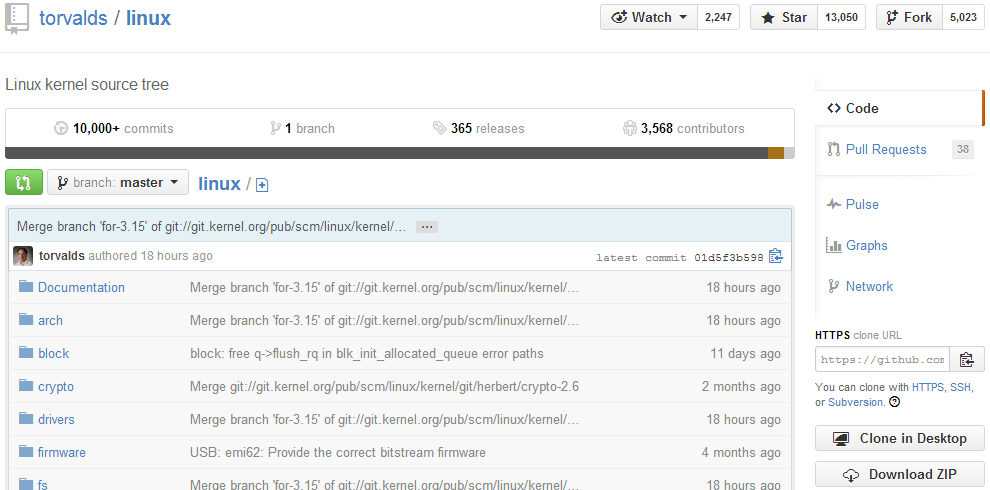
\includegraphics[width=0.98\textwidth]{./img/linux.png}
	\caption{Sample profile of a repository in GitHub}
	\label{fig:ghrepo}
\end{figure*}
With the advent of Web 2.0, online collaboration has become not only a part of internet experience but rather a necessity. People today are not just passive viewers of content but rather active contributors. Social networking sites such as Facebook and LinkedIn allow users to create both their personal and professional identities, respectively. Further, online communities such as blogs and wikis allow people to express opinions, carry out discussions, ask questions and answer queries, among other things. In addition, media sharing and hosting websites such as YouTube ensure fast propagation and easy accessibility of digital content.

Clearly, digital collaborations have revolutionized the way information is generated (i.e. through multiple sources), stored (social graphs and complex data types) and accessed (fast and ubiquitous) using just a web browser. This is also true for software development. Recently, platforms such as SourceForge, GitHub, BitBucket and CodePlex have experienced a rise in popularity. They are also referred to as social coding platforms i.e. development environment that encourages formal and informal collaboration on software projects providing opportunities for discussion and sharing. Open Source Software (OSS) in particular has experienced a rise in popularity. These open source projects are licensed to be freely modified and distributed and hence are often developed publicly where multiple developers collaborate to add or modify functionality.

The social aspects of OSS development provides insight into the dynamics of collaborations and opens interesting opportunities for research. Several studies throw light on what drives people towards OSS. Some of these factors include personal need for software \cite{Raymond1999}, creative stimulation \cite{lakhani2005}, learning \cite{Lakhani2003}, gift-giving intentions \cite{Zeitlyn2003} and significant returns on contribution \cite{ghosh2005}. Even though the developers have these intentions in mind, they seldom have any explicit metric to measure such factors. In the absence of such information developers indirectly assess the reputation of a project or a developer based on several other factors. For instance, number of followers of a developer can be indicative of their reputation in the coding community.

In this paper we will focus on collaborations between software developers, ``Social Coding'' and OSS development. We will discuss how these collaborations function by analysing one of the most popular social coding website - GitHub \cite{GitHub}. We are particularly interested in studying what motivates a developer to contribute into a project. The large amount of projects that a developer can join and contribute seems overwhelming. Yet, somehow, some of the projects seem to be more attractive to developers and have larger communities that are willing to  contribute to their development. A simple intuition of this phenomenon would be that popular projects attract developers simply because they are popular, like a snowball effect.

While this might be true for some projects, various counterexamples can be found in which a project quickly gathers a significant following, with no obvious reason. Our study will focus on analyzing the social network of GitHub and provide some answers to the following questions:

\textbf{Q1:} What is a typical contributor of a project?

\textbf{Q2:} Why do people follow specific projects?

We believe that by answering these questions we can help developers build a following to their projects. The remainder of our paper is structured as follows: In section 2 we will discuss similar factors that can affect collaboration decisions and reputation by reviewing some of the previous work that has been done in the field. Section 3 presents the data collected from Github and use it to answer Q1. In section 4, we analyze some trends on the data and use them to answer Q2. In section 5, we discuss some threats to the validity of our work. Finally, in section 6 we present our conclusions.


\section{Related Work}
\label{sec:related}

\cite{Thung2013} investigates the network structure of social coding in GitHub. In this study, they try to measure the strength of a) relationships among different projects and b) relationship between the developers. For this, they create network graphs of 30,000 projects randomly sampled from a set of 1,00,000 projects returned by the GitHub API and then randomly select 30,000 developers from these projects. This data is used to create two networks - A project-project network and a developer-developer network. In the project-project network each node of the network is a project and two projects are connected if they have at least one common developer. A weight is associated to each edge which signifies the number of developers that work on both the projects. In similar way the developer-developer network is constructed where nodes represent the developers and an edge is drawn between two developers when they work together on at least one project. Weight in this network represents the number of projects the two developers have worked upon together. These graphs are then analysed on three network characteristics - 1) Node degree 2) Network diameter and 3) Average shortest path using methodologies mentioned in \cite{Surian2010}. The authors also use the PageRank algorithm on these networks to find out the most influential projects and developers. The results show that the project networks are more interconnected than human networks and that social coding enables substantially more collaboration among developers.

In \cite{Dabbish2012}, the effect and value of ``transparency'' on people's inferences and decisions is analysed. This study is based on \cite{weiner2013}, in which it is claimed that ``awareness about the activities of user behavior on a social website enables other users on the network to draw inferences''. They performed a series of 24 semi-structured interviews with GitHub users where they were asked about the inferences they make about a user or a project and whether these inferences influence the projects or the people they follow. As expected, a rich set of inferences were made mostly based on 4 visual cues namely volume of activity, sequence of actions over time, attention to artifacts and people and the detail of information about an action. Each of these cues revealed a different type of information to the user making the inferences. For example, one of the users said that commits on a project revealed direction and intent of the contributor.

\section{Implementation}

\subsection{Platform}
\begin{figure}
\includegraphics[keepaspectratio, width=0.35\textheight]
{../presentation/img/architecture-diagram.png}
\caption{Architecture of our current platform. Clients are aware of the partition that
holds the initial vertex of a query. The server that accepted the request becomes the
coordinator, communicates with other servers, and replies to the client with a full
answer}
\label{fig:architecture}
\end{figure}

Our implementation of the graph database system can be seen on Figure
\ref{fig:architecture}. Our current platform implements hash partitioning due 
to its simplicity. All components have to include the partition manager in order
to know where to submit the requests. One major advantage of this scheme is that
clients will see reduced latencies, because they can communicate directly to the
partition that is holding a vertex.

Each server uses MySQL as a stand-alone database instance (each instance is
unaware of other instances). Every time a server accepts a request from a client,
it becomes the coordinator for that query and will likely communicate with
other servers in order to provide an answer to the client. Before going remotely,
the coordinator will try to fully satisfy the request locally, with the help of the cache.

Finally, the query execution layer implements one of the query processing
techniques discussed in Section \ref{sec:distributedqueryproc}.

\subsection{Cache}

We implemented caches that run at the vertex granularity -- get, put and
eviction calls work with one vertex at a time. The first cache policy
that we used is Least Recently Used (LRU); the same policy employed in TAO.
The second policy employed is ARC \cite{Nimrod03ARC}. Our implementation of ARC
is based on modifying LRU according to the description in \cite{Nimrod03OUL}.
The third policy comes from an algorithm of our own: Local Connected Cache (LCC).

\subsubsection{Local Connected Cache}

\begin{figure}
	\includegraphics[keepaspectratio, width=0.35\textheight]
	{./img/LCC.png}
\caption{LCC Placement Policy: It first assigns a score of 8 to vertex 6789. It
then inserts this vertex into LRU Level 8 -- a cache working under LRU policy
for all vertices with score of 8. For evictions, LCC will evict the least-recently
used vertex from LRU Level 0.}
\label{fig:lcc}
\end{figure}

LRU and ARC are unaware of the underlying structure of the data. Because these
caching policies dismiss all information about edges, they are unable to exploit
other features that are particular to graph databases.

Local Connected Cache (LCC) works as a multi-level LRU cache. It assigns a
score to each vertex. For our current implementation of LCC, the score is given
by the number of in-edges a remote vertex has with respect to local vertices.
LCC then proceeds to place the vertex on the appropriate level: Given a score {\it s}
for vertex {\it v}, LCC puts {\it v} in LRU level {\it s} (Figure~\ref{fig:lcc}).

LCC's eviction policy is straightforward. It evicts the least-recently used vertex from
the lowest level cache. Our intuition behind this algorithm is that the probability of
a vertex being requested in the future increases with the size of the neighborhood
of the vertex in a given partition. The algorithm tries to evict first the vertices that
have a smaller neighborhood. Additionally, evictions are O(1) with respect to cache
size, minimizing the amount of contention between threads. This point is important,
as one of our failing caching algorithms scanned over the entire cache resulting in
contention for critical sections becoming the bottleneck.

\subsection{Distributed Query Processing}
\label{sec:distributedqueryproc}

We have implemented two types of queries:
\begin{enumerate}
\item $h$-hop Random Walk (hRW): Starting at a vertex, randomly choose one of
its outgoing edges, and walk to that vertex. Repeat this, until $h$ edges have
been walked, and return the end vertex.

\item $h$-hop Neighborhood Retrieval (hNR): Starting at a vertex, return all the
vertices that are at a distance of at most $h$ hops.
\end{enumerate}

We discuss three models for implementing distributed query processing. In our
project, we used the Single Source Query Coordinator model.

% Sample execution of 3-NR in all the query processing models.
\begin{figure*}
\centering
	% The original graph
	\begin{subfigure}{0.2\textwidth}
	\scalebox{0.7}{
		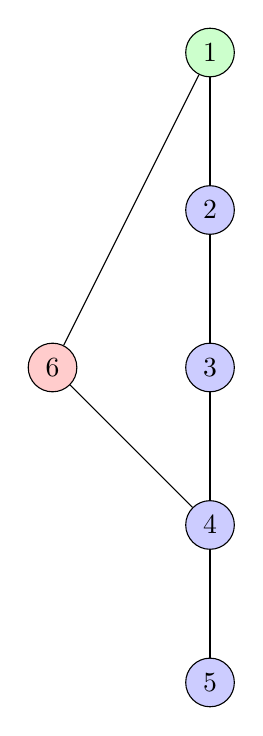
\begin{tikzpicture}
		[
			p1/.style={circle, draw, fill=green!20},
			p2/.style={circle, draw, fill=blue!20},
			p3/.style={circle, draw, fill=red!20},
		]

		% Nodes
		\foreach \style/\name/\x/\y in
		{
			p1/1/2/8,
			p2/2/2/6,
			p2/3/2/4,
			p2/4/2/2,
			p2/5/2/0,
			p3/6/0/4
		}
			\node[\style] (\name) at (\x,\y) {\name};

		% Edges
		\foreach \u/\v in
		{
			1/2,
			1/6,
			2/3,
			3/4,
			4/5,
			6/4}
			\draw (\u) -- (\v);

		\end{tikzpicture}
	}
	\caption{\label{subfig:graph}}
	\end{subfigure}
	~
	% Single Source Query Coordinator Model
	\begin{subfigure}{0.2\textwidth}
	\scalebox{0.7}{
		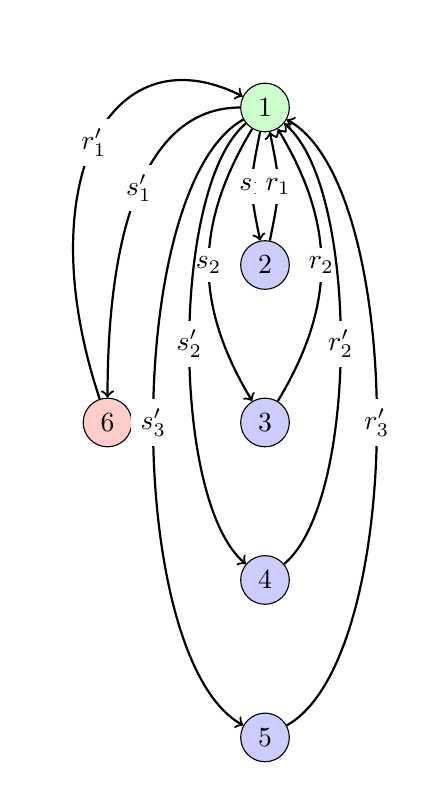
\begin{tikzpicture}
		[
			p1/.style={circle, draw, fill=green!20},
			p2/.style={circle, draw, fill=blue!20},
			p3/.style={circle, draw, fill=red!20},
		]

		% Nodes
		\foreach \style/\name/\x/\y in
		{
			p1/1/2/8,
			p2/2/2/6,
			p2/3/2/4,
			p2/4/2/2,
			p2/5/2/0,
			p3/6/0/4
		}
			\node[\style] (\name) at (\x,\y) {\name};

		% Requests
		\foreach \u/\v/\a/\b/\text in
		{
			1/2/{( 1.8,  7  )}/{( 1.8,  7  )}/$s_1 $,
			2/1/{( 2.2,  7  )}/{( 2.2,  7  )}/$r_1 $,
			1/6/{( 0.5,  8  )}/{( 0  ,  6.5)}/$s_1'$,
			6/1/{(-1  ,  7  )}/{( 0  ,  9  )}/$r_1'$,
			1/3/{( 1.1,  6.5)}/{( 1.1,  5.5)}/$s_2 $,
			3/1/{( 2.9,  5.5)}/{( 2.9,  6.5)}/$r_2 $,
			1/4/{( 0.8,  7  )}/{( 0.8,  3  )}/$s_2'$,
			4/1/{( 3.2,  3  )}/{( 3.2,  7  )}/$r_2'$,
			1/5/{( 0.2,  7  )}/{( 0.2,  1  )}/$s_3'$,
			5/1/{( 3.8,  1  )}/{( 3.8,  7  )}/$r_3'$
		}
			\draw[thick, ->] (\u) .. controls \a and \b .. node[fill=white] {\text} (\v);

		\end{tikzpicture}
	}
	\caption{\label{subfig:sscquery}}
	\end{subfigure}
	~
	% State Passing Query Coordinator Model
	\begin{subfigure}{0.2\textwidth}
	\scalebox{0.7}{
		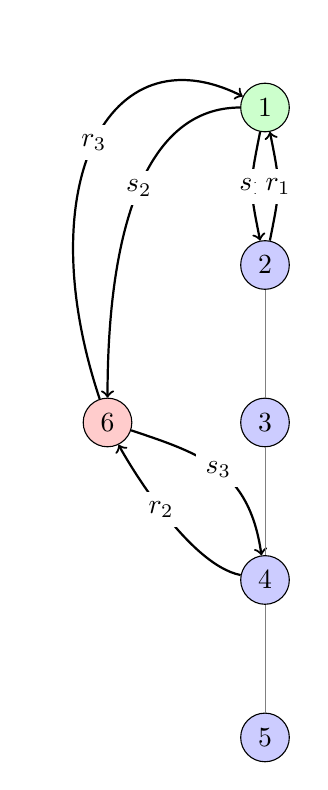
\begin{tikzpicture}
		[
			p1/.style={circle, draw, fill=green!20},
			p2/.style={circle, draw, fill=blue!20},
			p3/.style={circle, draw, fill=red!20},
		]

		% Nodes
		\foreach \style/\name/\x/\y in
		{
			p1/1/2/8,
			p2/2/2/6,
			p2/3/2/4,
			p2/4/2/2,
			p2/5/2/0,
			p3/6/0/4
		}
			\node[\style] (\name) at (\x,\y) {\name};

		% Requests
		\foreach \u/\v/\a/\b/\text in
		{
			1/2/{( 1.8,  7  )}/{( 1.8,  7  )}/$s_1$,
			2/1/{( 2.2,  7  )}/{( 2.2,  7  )}/$r_1$,
			1/6/{( 0.5,  8  )}/{( 0  ,  6.5)}/$s_2$,
			6/1/{(-1  ,  7  )}/{( 0  ,  9  )}/$r_3$,
			6/4/{( 1.2,  3.6)}/{( 1.8,  3.4)}/$s_3$,
			4/6/{( 1  ,  2.2)}/{( 0.2,  3.6)}/$r_2$
		}
			\draw[thick, ->] (\u) .. controls \a and \b .. node[fill=white] {\text} (\v);

		% Edges
		\foreach \u/\v in
		{
			2/3,
			3/4,
			4/5}
			\draw[help lines] (\u) -- (\v);

		\end{tikzpicture}
	}
	\caption{\label{subfig:spcquery}}
	\end{subfigure}
	~
	% Distributed State and Query Coordinators Model
	\begin{subfigure}{0.2\textwidth}
	\scalebox{0.7}{
		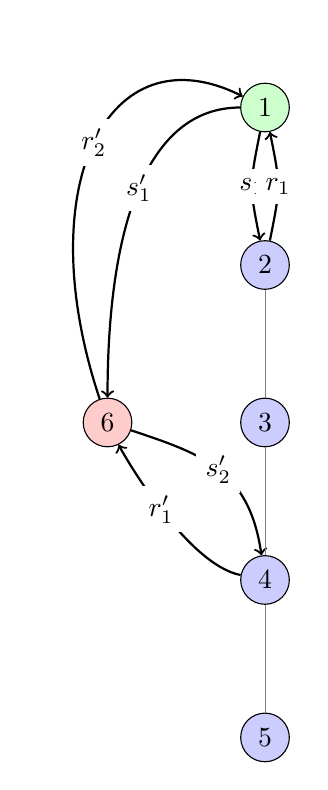
\begin{tikzpicture}
		[
			p1/.style={circle, draw, fill=green!20},
			p2/.style={circle, draw, fill=blue!20},
			p3/.style={circle, draw, fill=red!20},
		]

		% Nodes
		\foreach \style/\name/\x/\y in
		{
			p1/1/2/8,
			p2/2/2/6,
			p2/3/2/4,
			p2/4/2/2,
			p2/5/2/0,
			p3/6/0/4
		}
			\node[\style] (\name) at (\x,\y) {\name};

		% Requests
		\foreach \u/\v/\a/\b/\text in
		{
			1/2/{( 1.8,  7  )}/{( 1.8,  7  )}/$s_1 $,
			2/1/{( 2.2,  7  )}/{( 2.2,  7  )}/$r_1 $,
			1/6/{( 0.5,  8  )}/{( 0  ,  6.5)}/$s_1'$,
			6/1/{(-1  ,  7  )}/{( 0  ,  9  )}/$r_2'$,
			6/4/{( 1.2,  3.6)}/{( 1.8,  3.4)}/$s_2'$,
			4/6/{( 1  ,  2.2)}/{( 0.2,  3.6)}/$r_1'$
		}
			\draw[thick, ->] (\u) .. controls \a and \b .. node[fill=white] {\text} (\v);

		% Edges
		\foreach \u/\v in
		{
			2/3,
			3/4,
			4/5}
			\draw[help lines] (\u) -- (\v);

		\end{tikzpicture}
	}
	\caption{\label{subfig:dscquery}}
	\end{subfigure}
\caption{\ref{subfig:graph}: A graph with 3 partitions. We show the execution of
a 3-hop Neighborhood Search in the 3 query models presented in
Section~\ref{sec:distributedqueryproc}, starting at vertex $1$.
\ref{subfig:sscquery}: Getting a remote vertex always requires a network call.
\ref{subfig:spcquery}: State is passed to the partition where the query would
normally flow. Each partition is visited in sequence.  \ref{subfig:dscquery}:
State is maintained in a distributed manner. Control can flow in parallel to
each partition.}
\label{fig:querymodels}
\end{figure*}

\subsubsection{Single Source Query Coordinator}
\label{sec:singlesourcequerycoord}

This model is agnostic of partitioning. Queries are executed at the starting
partition as if all vertices are local. When a remote vertex is required because
of some edge traversal, it is retrieved from the remote partition with a network
call. The advantage of this model is that it abstracts query execution from data
layout, so that query state is maintained at a single source, that can always
coordinate traversals in an optimal way.

An example of this execution can be seen in Figure~\ref{subfig:sscquery}, when
answering the 3NR query starting at vertex $1$. Since each vertex is remote,
they are brought over the network in iterative fashion. Vertices $\{2, 6\}$ can
be brought in parallel, with separate requests $s_1$ and $s_1'$.

The disadvantage of this model is the amount of network requests that need
to be made -- 5 in Figure~\ref{subfig:sscquery}. Even for vertices such as
$\{4,5\}$ that are located on the same partition and traversed together, we
require sending two network requests to retrieve them. This inability of
accessing nodes that are co-located also hurts in terms of caching. A remote
partition that is accessed by a query, and stores intermediate results for that
query in its cache, cannot use those results.

\subsubsection{State Passing Query Coordinator}
\label{sec:statepassingquerycoord}

This model passes the current state of a query to the remote partition required
to be visited next because of an inter-partition edge. This is used to reduce
the amount of network calls required for traversing edges. For example in
Figure~\ref{subfig:spcquery}, while satisfying the 3NR query, and traversing the
edge $(1, 2)$, we pass all the current visited vertices, as the state of the
query, to the blue partition. There, the edges $(2, 3)$ and $(3, 4)$ are
traversed locally, and state is returned to the green partition, which continues
its execution.

The disadvantage of this model is that, although the number of network messages
decreases, the amount of data sent per network message increases -- sometimes
considerably depending on the graph layout. Furthermore, queries are no longer
independent of the partitioning of data. For example, in
Figure~\ref{subfig:spcquery}, vertex $4$ is visited twice as part of the 3NR
query. Once when traversing edge $(3, 4)$, when it is at a distance of 3-hops
from $1$, and once when traversing edge $(6, 4)$, when it is at a distance of
2-hops from $1$. As such, queries like 3NR which are breadth-first search in
nature, need to be modified to fit the iterative deepening style of traversal.
Lastly, this model requires sequential execution, despite the fact that multiple
edges can be traversed in parallel in the original query, as seen in
Section~\ref{sec:singlesourcequerycoord}. This is due to the fact that state
passes along the edges.

\subsubsection{Distributed State and Query Coordinators}
\label{sec:distributedstatequerycoord}

This model maintains a distributed state of the query at the partitions that are
accessed. This is achieved by generating unique query IDs, which are passed to
remote partitions together with the continuation of the query. Each partition
tags the vertices that are visited by a query with the query ID and the
appropriate state determined by the query continuation.

For example, in Figure~\ref{subfig:dscquery}, while executing the 3NR query,
when edge $(1, 6)$ is traversed, the query ID, the number of remaining
hops (2) and the current hop count (1) is passed to the red partition. This is
used to tag vertex $6$ as being at distance $1$ within the specified query, and
a continuation follows while traversing edge $(6, 4)$.

The benefit of this model is that minimal information needs to be passed during
network calls -- the query ID and state that is constant in size. This is in
contrast to the previous model, where state was proportional to the query result
size. Furthermore, in this model, edges can be traversed in parallel, as state
is maintained in a distributed manner by each partition. In the provided
example, edges $(1, 2)$ and $(1, 6)$ can be traversed in parallel.

The disadvantage of this approach is that a vertex such as $4$ can be visited
twice, with different distance metrics, depending on the ordering of the
parallel requests. Thus, like in the previous mode, a query needs to be modified
since it is no longer independent of the partitioning and traversal schema.

\section{Data and Queries}

We make use of LinkBench for generating our graph.  The probability of a node
having some number of edges follows a Zipfian distribution. This means that the
probability of a node having some degree decreases exponentially as the degree
increases.

% read only
% reads of nodes are Zipfian
We re-use their application to generate our workloads. The workloads
that LinkBench see are after cache. As a result, we attempt to approach a
pre-cache workload by adjusting the parameters to LinkBench's distributions.
Second, we assume a read only workload, because TAO and LinkBench observed
primarily reads. This allows us to focus on cache optimizations. The focus of
this paper is not cache invalidation and isolation. The probability of a user
being read some number of times also follows a Zipfian distribution. What this
means is that the probability of a node being read some number of times
decrease exponentially with respect to the number of reads.

% 2-hop query
% random walk queries
% return all nodes
Since photos, status updates, and people are nodes in the graph, queries requesting
all of the photos that a person's friends posted become two hop. One hop to
determine the person's friends, and a second hop to determine their friends' photos.
As a result, we modify the LinkBench workload generator to perform 2-hop queries.
LinkBench only generates 0-hop queries like: getting a node, getting the edges of a
node, and getting an edge. Additionally, we include random walk queries that
represent a user following edges starting from their starting node.

% Result limit
% no history
LinkBench limits the number of nodes returned based on their timestamp. The
reason is that a person would be interested in the most recent events. Since
less than 3\% of queries returned more than 100 vertices, we limit the number of
vertices returned to 100. Secondly, after retrieving the initial vertices, the
probability of reading historically for old vertices was 0.96\%. We removed
these from our workload because a small amount of queries asked for it.


\section{Results}
\begin{table}
\centering
\begin{tabular}{ | c | c | c | c | }
	\hline
	\multicolumn{2}{|c|}{Project} & \multicolumn{2}{|c|}{Owner} \\ \hline
	Ranking & Followers & Ranking & Followers \\ \hline
	1 & 30,229 & 111,278 & 2 \\ \hline
	2 & 28,594 & 193,670 & 0 \\ \hline
	3 & 24,682 & >1,000 & -  \\ \hline
	4 & 23,830 & 21 & 4,161 \\ \hline
	5 & 22,167 & 193,670 & 0 \\ \hline
	6 & 21,227 & 111,278 & 2 \\ \hline
	7 & 17,485 & 12 & 5,213 \\ \hline
	8 & 16,543 & >1,000 & - \\ \hline
	9 & 15,648 & 87 & 1,406 \\ \hline
	10 & 15,235 & 33,877 & 12 \\ \hline
\end{tabular}
\caption{Relation between followers of a project (stars) and followers of the owner of the project. }
\label{tbl:owner}
\end{table}
\label{sec:results}

To answer Q2, we formulated four hypothesis in an attempt to characterize the motivations behind developers following a project. The hypothesis are: (i) popularity grows because the owner of the project is popular; (ii) popularity grows because the number of popular contributors working on it; (iii) popularity is affected by the programming language; (iv) popularity is determined by the category that it belongs to. We now present the results obtained for each of the four hypothesis:

\subsection{Owner}

The owner of the project is the user who originally created and published it on GitHub. We hypothesize that the popularity of the owner influences the popularity of the project he/she owns. A relation was made between the number of stars of the project and the number of followers of the owner. We started by analyzing the behaviour of the 100 most popular projects and their owners, hoping to find a positive correlation. Table \ref{tbl:owner} shows no concrete evidence about the 10 most popular projects. We could not find information about some of the owners in our database (rows 3 and 8), thus we can only affirm that they are not between the 1,000 most popular users (see Section \ref{sec:collection} for details).

A more general case is shown in Figure \ref{fig:owner}. It can be seen that a large number of popular projects have owners with little following. Finally, for the complete set of projects included in our sample, the correlation between owners and projects is 0.01, using Pearson's correlation coefficient. Therefore, we conclude that there is no correlation at all between stars and followers.
\begin{figure}
	\centering
	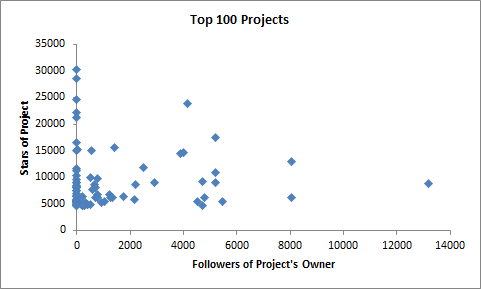
\includegraphics[width=0.45\textwidth]{./img/top100Owner.png}
	\caption{Relation between popularity of the project (given by stars) and the popularity of the project's owner (given by followers).}
	\label{fig:owner}
\end{figure}

\subsection{Contributors}

A contributor of a project is a user who actively participates in its development. We hypothesize that the involvement of one or more popular users on a project will influence on the project's popularity. In order to prove/disprove this, we collected the UserID of all contributors that belong to some of most popular projects. Due to the large amount of information and API restrictions, we could only collect the contributors of the one thousand most popular projects. We wanted to know how many popular users were contributing to such projects.

Table \ref{tbl:contributors} shows the relation between contributors and popularity of projects. We grouped the 100 and 1,000 most popular users and projects and determined the involvement of each. It shows, for example, that only 48 of the top 100 users are involved in the top 100 projects. Even more interesting, these 48 users are working on 18 of such projects. In other words, 82\% of the 100 most popular projects have no involvement of popular users. On the other side of the table, we have that almost a half (43\%) of the 1K most popular users are contributing to a quarter (22\%) of the 1K most popular projects. Because there's a large number of projects with no involvement of popular users, we dismiss this hypothesis as well.
\begin{table}
\centering
\begin{tabular}{ | l | c | c | c | c | }
	\hline
	\- & \multicolumn{2}{|c|}{Top 100 Projects} & \multicolumn{2}{|c|}{Top 1K Projects} \\ \hline
	\multicolumn{1}{|c|}{Users} & Uq Proj. & Uq Users & Uq Proj. & Uq Users \\ \hline
	Top 100 & 18 & 48 & 113 & 65 \\ \hline
	Top 1K & 23 & 286 & 222 & 431 \\ \hline
\end{tabular}
\caption{Relation between contributors and popularity of a project. Uq stands for Unique.}
\label{tbl:contributors}
\end{table}

\subsection{Programming language}

The programming language of a project can be a difficult choice for the owner. The owner probably wants to appeal to a broad audience by choosing a popular language. But sometimes there is no choice and the language is given by the specification of the project. For example, an Android app will have to be written with Java. For hypothesis 3, we wanted to determine the impact in popularity for choosing a specific programming language. We observed 128 different programming languages on our sample and a ``None'' language, which basically means that the project is missing that information. The metric we used for validating the hypothesis was the percentage of projects written in the same language that have more than 2,500 followers, a metric which we call the language success rate. We note that 2,500 followers is slightly lower than the average number of followers for the 1K most popular projects (See Table \ref{tbl:toprepos}), so we consider it a good popularity threshold.

The results are given in Table \ref{tbl:languages}. The total number of projects is given by P. F/P is the average number of followers per language and F > {$ \tau $} is the number of projects that have more than {$ \tau $} ({$ \tau $} = 2,500) followers. The last column is the language success rate. Several observations can be made. First, the two languages with the most projects (Javascript and Ruby) are also the ones that have the most projects above the {$ \tau $} threshold. Julia has a 50\% success rate, but its sample size is too little to make a reasonable generalization. Finally, the languages with a high average on followers are CSS, Rust, Julia and TypeScript, which are also the ones that have the highest success rate.

The correlation within the number of projects and the success rate is of 0.53, when the ``None'' language is removed. If we consider the ``None'' language, this correlation falls to 0.27. This tells us that there is some correlation between the most popular programming languages and the amount of projects that the language will have above the threshold {$ \tau $}. The only problem is that the success rates are so low or, in the case of Julia, the sample size is so little, that no positive conclusion can be made about the programming languages. So we also dismiss this hypothesis.
\begin{table}
\centering
\begin{tabular}{ | l | c | c | c | c | }
	\hline
	\multicolumn{1}{|c|}{Language} & P & F/P & F > {$ \tau $} & (F > {$ \tau $}) / P \\ \hline
	None & 171,894 & 1.89 & 3 & 0.002\% \\ \hline
	C & 39,716 & 8.55 & 15 & 0.038\% \\ \hline
	C\# & 15,240 & 7.84 & 1 & 0.007\% \\ \hline
	C++ & 26,071 & 7.49 & 5 & 0.019\% \\ \hline
	Clojure & 4,407 & 12.94 & 1 & 0.023\% \\ \hline
	CoffeeScript & 1,427 & 40.40 & 3 & 0.210\% \\ \hline
	CSS & 1,857 & 74.27 & 11 & 0.592\% \\ \hline
	Java & 57,953 & 6.76 & 11 & 0.019\% \\ \hline
	JavaScript & 106,987 & 17.40 & 107 & 0.100\% \\ \hline
	Julia & 2 & 1,780.00 & 1 & 50.000\% \\ \hline
	Objective-C & 20,784 & 21.87 & 21 & 0.101\% \\ \hline
	Perl & 43,808 & 2.72 & 1 & 0.002\% \\ \hline
	PHP & 54,337 & 8.39 & 12 & 0.022\% \\ \hline
	Python & 71,942 & 9.46 & 24 & 0.033\% \\ \hline
	Ruby & 173,960 & 8.89 & 51 & 0.029\% \\ \hline
	Rust & 62 & 76.18 & 1 & 1.613\% \\ \hline
	Shell & 14,158 & 9.68 & 7 & 0.049\% \\ \hline
	TypeScript & 92 & 99.39 & 1 & 1.087\% \\ \hline
	VimL & 13,961 & 9.31 & 8 & 0.057\% \\ \hline
\end{tabular}
\caption{Relation between programming languages and popularity of a project. The value chosen for {$ \tau $} was 2,500.}
\label{tbl:languages}
\end{table}
\subsection{Categories}
Our final hypothesis involves the categorization of projects. We claim that developers follow a project based on its intended usage. So, for example, 3D rendering software will usually have more followers than unit testing tools. We took the 100 most popular projects and visited their websites and repositories in order to find what their functionality is. We then assigned a broad category which we thought best described the project. The results are shown in Figure \ref{fig:categories}. We included the programming language as well, in order to better understand the distribution of the projects.

The most common categories are framework and widget / plugin. Examples of frameworks are JQuery and Symphony. Examples of widgets / plugins are FileUploader and JavaScript PDF reader. Also noteworthy to mention is that JavaScript frameworks and widgets / plugins are, by far, the most common types of project found on this phase of the study. Other categories found were front-end generators, libraries and networking tools. We believe this shows a trend about what kind of projects are users interested in following, i.e. web development productivity tools. This certainly shows the best results out of the four hypothesis we made. But, because the sample size is so small, we cannot generalize these results. In order to claim with some level of certainty that these categories correlate to the popularity of a project, we need to determine, out of all the frameworks hosted on GitHub, the percentage of successful ones. In other words, we suggest applying the same success rate metric we used for evaluating the programming languages.
\begin{figure*}[ht]
	\centering
	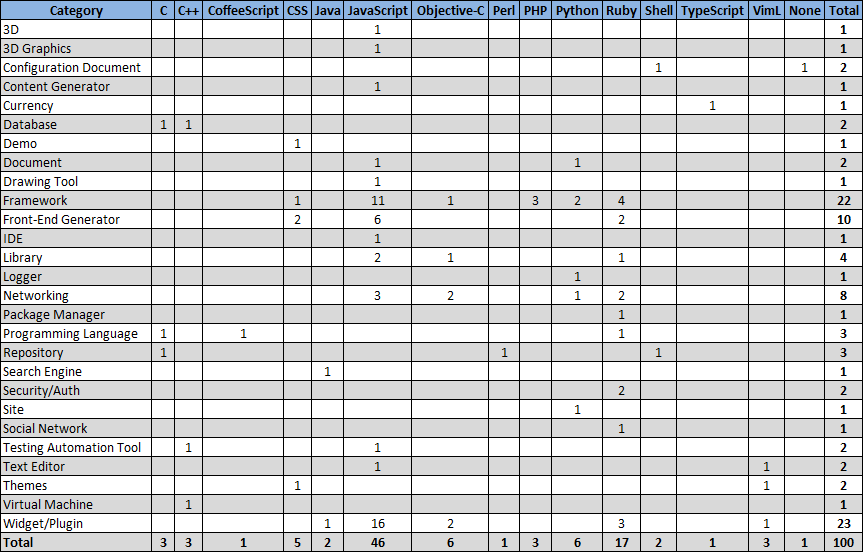
\includegraphics[width=\textwidth]{./img/categories.png}
	\caption{Categories of the 100 most popular projects, grouped by programming language. The most popular category is Widget/Plugin and 16 out of the 23 projects that fall within this category are developed using Javascript.}
	\label{fig:categories}
\end{figure*}


\section{Future Work}

% Query passing model
Due to the poor cache performance of using a query coordinator model, and the
explanation for its poor performance, the next steps would be to look at
implementing the second approach that we proposed where the query is passed on
to further be processed by other hosts. This will allow queries to take
advantage of another machine's cache. In the coordinator model, the number of
remote calls we do only depends on the starting machine's cache. The reason we
initially began with a coordinator model for this paper was for ease of
implementation. We attempted a naive version of the query passing model, but it
did not perform well due to CPU usage.

% Relaxing assumptions:
% - read only
% - no history
We made simplifying assumptions to allow us to focus on the caching
implementation. In the future, the assumptions need to be relaxed. We assumed a
read only workload, allowing us to postpone investigating isolation and cache
invalidation. Secondly, we do not consider a client requesting further history
after the first 100 vertices.

We also wish to extend the LCC algorithm and try different scoring functions. We
initially tried to assign a score to a vertex based on how well it was connected to
other vertices already in cache. The intuition behind this algorithm is that vertices
that are well connected amongst each other will usually be accessed together, so
it will be convenient to keep them together in cache. The difficulty from this scoring
function arises from the fact that scores need to be updated every time a vertex
enters or leaves the cache, possibly modifying all elements on cache. We have
several optimizations in mind but we leave them for future versions.

For random walk, we need to test with different and varying depths to better
assess the quality of each cache.

Finally, as stated before, we believe that results can be extended to other datasets
under different workloads. We plan to evaluate our caching algorithms under
different datasets, like Orkut or RDF data.


\section{Conclusions}

Scaling graph databases can be challenging, especially when dealing with highly
interconnected graphs.  We explored different, well-known caching algorithms
that allowed us to replicate data across partitions based on Zipfian read
workloads.  We also introduced a novel caching algorithm, Local Connected Cache
(LCC), as a way to exploit the underlying nature of graph data. LCC is a
multi-level LRU caching algorithm that assigns scores to vertices based on how
well connected they are to other local vertices on a given partition.

Although this algorithm highly favors immediate (1-hop) neighbours, we
showed that it does not perform well for k-hop neighbours and that is highly
dependent on the query access model that the underlying database implements.
We believe LCC will improve performance significantly if allowed to work with
intermediate caches, a direction we wish to pursue on future versions of the
platform.

We then compared two other caching algorithms, LRU and ARC, and showed
that ARC provides better performance in all three metrics that we collected.


\bibliographystyle{plain}
\bibliography{paper}
\end{document}
